\chapter{Mise en \oe{}uvre d'IITAMP} % (fold)
\label{cha:Mise en oeuvre d'IITAMP}

\begin{it}
Après la création d'IITAMP ainsi que l'élaboration de toute sa
documentation, je l'ai installé sur un serveur local chez un client pour
héberger la solution GeMa qui est développé par \emph{IdentIt}. J'ai eu
aussi l'opportunité de réaliser une vidéo d'utilisation de GeMa dans le
cadre d'une présentation par les responsables de l'entreprise cliente à
leurs salariés.
\end{it}

\section{Présentation de GeMa} % (fold)%{{{
\label{sec:Présentation de GeMa}

\lettrine{G}{eMa} est une solution de maintenance innovante alliant
RFID, mobilité et technologie Web. L'application embarquée sur
PDA,\footnote{\emph{Personal Digital Assistant} où assistant numérique
personnel.} permet la consultation des interventions à réaliser, la
saisie des rapports et l'accès aux données techniques nécessaires au bon
déroulement des travaux.

\begin{quotation}
\og{}Avec GeMa, le responsable de maintenance prépare depuis son poste
informatique les ordres de travaux pour lesquels il mandate un
intervenant sur site. Les techniciens, quant à eux, reçoivent en temps
réel leurs missions sur PDA qu'ils complètent grâce à une interface
ergonomique (menus déroulants, cases à cocher\dots). Les rapports ainsi
réalisés remontent instantanément sur le serveur. \fg{} M.~Dubourg.
\end{quotation}

Une intervention à réaliser sur un équipement : le technicien
l'identifie grâce à son étiquette RFID scannée par le PDA. Une anomalie
découverte lors d'un contrôle : le technicien la photographie grâce à
l'appareil numérique intégré. Un élément laissé sur place : le
technicien indique sa position sur site, grâce aux fonctions GPS de
GeMa. En temps réel, les responsables et/ou clients disposent
d'informations fiables et exploitables au travers d'historiques, de
statistiques, de bilans, d'alertes email ou via des échanges avec un
logiciel tiers. La figure~\ref{gema} en page~\pageref{gema} illustre
l'utilisation conventionnelle de l'application.

\begin{figure}
  \begin{center}
    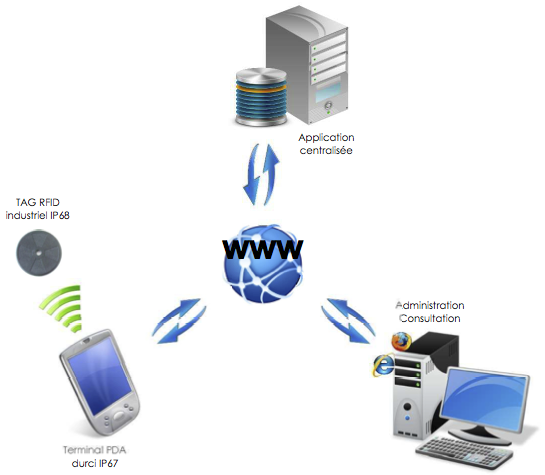
\includegraphics{images/gema.png}
    \caption{Schéma d'utilisation de GeMa via l'Internet.}
    \label{gema}
  \end{center}
\end{figure}
% section Présentation de GeMa (end)%}}}

\section{Mise en place de la solution} % (fold)%{{{
\label{sec:Mise en place de la solution}

Pour une interconnexion entre les sites, un dispositif de sécurité
impressionnant à été mis en place par Syngenta. En effet, ceux-ci
utilise la technologie VPN,\footnote{\emph{Virtual Private Network} ou
réseau privé virtuel.} qui permet d'obtenir une liaison sécurisée à
moindre coût.

Le réseau privé virtuel vise à apporter certains éléments essentiels
dans la transmission de données : l'authentification (et donc
l'identification) des interlocuteurs, la confidentialité des données via
le chiffrement (qui vise à les rendre inutilisables par quelqu'un
d'autre que le destinataire). La figure~\ref{vpn} illustre le principe
de ce type de connexion.

La mise en \oe{}uvre d'IITAMP ainsi que de GeMa s'effectuant dans
l'usine de Nerac près de bordeaux, le client nous à prêter un ordinateur
portable avec tout les outils nécessaire à la connexion à distance pour
éviter de me déplacer de Dunkerque jusqu'au site, ce qui représente à
peu près 600 kilomètres...

\begin{figure}
  \begin{center}
    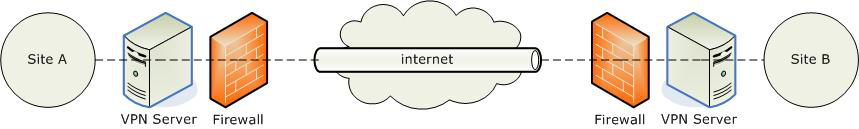
\includegraphics[scale=0.5]{images/vpn.png}
    \caption{Exemple de réseau privé virtuel entre deux sites.}
    \label{vpn}
  \end{center}
\end{figure}

\subsection{Harmonisation des systèmes d'informations} % (fold)%{{{
\label{sub:Harmonisation des systèmes d'informations}

Dans le cadre de cette mise en \oe{}uvre, le client veut récupérer les
données des interventions qui sont stockés dans la base MySQL de GeMa
dans leur système d'information qui possède une base de donnée SQL
Server. Cette duplication de donnée permet une intégration des
informations récoltés par GeMa dans le SI de l'entreprise à des fins de
traçabilité, ce qui permet à partir des autres logiciels du client de
faire des statistiques de production.

Pour cette duplication, il à fallu que je développe un script PHP qui
tout d'abord interroge la base de donnée de GeMa pour récupérer les
données, qui ensuite traite ses données pour les rendre compatibles à la
structure de la base du client ainsi qu'a la technologie SQL Server
utilisée et qui enfin insère ses données traités dans la base du client.

\subsection{Les tests} % (fold)%{{{
\label{sub:Les tests}

Comme nous l'avons vu, GeMa utilise la mobilité pour le rapport des
interventions. Pour tester si l'application GeMa fonctionne correctement
ainsi que le script de duplication de donnée, quelques tests furent
nécessaire. Étant donnée que le site de production n'est pas proche,
l'utilisation d'un émulateur de PDA au travers du réseau VPN fut
nécessaire.

Quelques problèmes sont apparu pendant la phase de debogage :
\begin{description}

  \item[Communication entre les bases :] XAMPP par défaut ne permet pas
    d'utiliser une base SQL Server, il à fallut que j'installe et
    configure le driver officiel de l'entreprise
    Microsoft pour permettre l'accès à la base de
    données.

  \item[Synthaxe invalide pour SQL Server :] Une habitude est ancrée
    dans l'utilisation du logiciel libre MySQL qui est de forcer
    l'encodage des caractères en UTF-8 afin d'éviter de futur problèmes.
    Cette manipulation ce fait via une requête SQL que l'on place dans
    le constructeur de la classe qui sert à instancier l'objet de
    connexion à la base de données. Comme les habitudes ont la vie dure,
    j'ai copié/collé un constructeur sans y prêter attention, cependant
    SQL Server ne connait pas cette syntaxe SQL. GeMa étant pourvu d'un
    système d'alerte par mail, M.~Dubourg recevait un courriel à 5
    minutes d'intervalles lorsque l'émulateur d'assistant personnel
    lançait la synchronisation distante avec le serveur\,
    \footnote{fonction de synchronisation automatique de GeMa Mobile
    lorsque il est sur son socle.}, sont client mail à bien entendu
    déplacer l'expéditeur entant que spam au bout de plusieurs reprises.
    Ne fermant pas l'émulateur la nuit pour éviter d'avoir à le
    relancer, une quantité impressionnante de mail m'a été annoncé
    quelques jours plus tard lorsque le cogérant à inspecté sa boite à
    pourriels.

  \item[Obligation de renseigner tous les champs :] L'ancien système de
    relevés ce faisant à l'aide d'un papier/crayon puis par l'ajout de
    ses annotations dans un fichier Excel, lorsqu'un champ n'avait
    aucune valeur, un zéro lui était attribué. En inspectant les données
    de la base SQL Server, je me suis rendu compte que mon script quant
    à lui n'insérait rien lorsqu'il n'y avait pas de valeur. J'en ai
    déduit qu'aucune règle de gestion n'avait été crée afin d'empêcher
    la non-saisi. J'ai donc été obligé d'inscrire cette règle via le
    code\,\footnote{c'est la base du client, je n'ai pas à intervenir
    dessus même si elle me parait mal conçu.} alors que la bonne méthode
    est habituellement de le faire via une option lors de la création de
    la base.

\end{description}
% subsection Les tests (end)%}}}
% subsection Harmonisation des systèmes d'informations (end)%}}}
% chapter Mise en oeuvre d'IITAMP (end)
